%=======================================
%
% $Id$
%
%=======================================

\documentclass[12pt]{article} 
\usepackage{amssymb} 	% additional symbols (there are more packages)
\usepackage{amsmath}
\usepackage{graphicx}
\usepackage{color}

%\usepackage{hyperref}
\usepackage[pagebackref=true,breaklinks=true,letterpaper=true,
colorlinks=true,urlcolor=blue,citecolor=blue,bookmarks=false,
pdfborder={0 0 0}]{hyperref}

\usepackage{anysize} 		% margin package sets tighter margins
\marginsize{1.0in}{0.8in}{0.2in}{1.0in} 	% small margins - left, right, top, bottom

\begin{document}
%\author{Yekaterina Kharitonova}
%\title{Title}
%\maketitle

\hfill Last modified: \today \\%by Yekaterina Kharitonova

\noindent
{\Large \bf Getting started with Bisque}\\ 

This document outlines steps needed to get started with Bisque~\cite{Bisque}.
%(\url{http://www.bioimage.ucsb.edu/downloads/Bisque%20Database}). 

% -----------------------------------------------
\section{Preliminary steps}
\label{sec:Preliminary}
\subsection{iPlant account}
\label{sec:iPlant_account}

Use Trellis~\cite{Trellis}
to create an account and log-in to the dashboard.
One of the services listed under ``Available services" is Bisque.

\begin{figure}[h]
\centering
  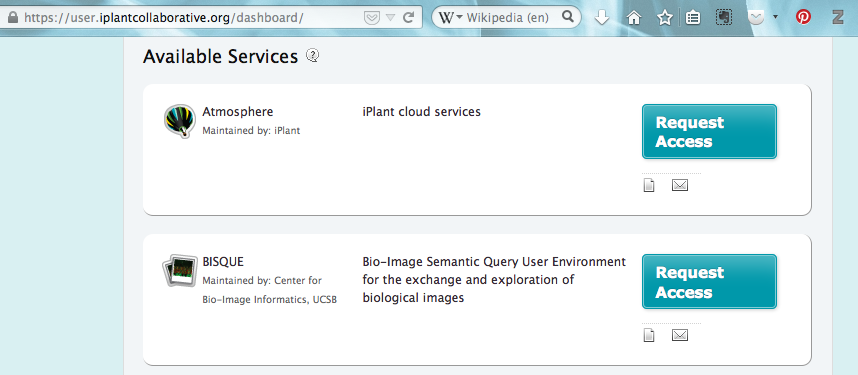
\includegraphics[width=0.6\linewidth]{./figures/available_services.png}
  \label{fig:available_services}
  \caption{The services available through your Trellis dashboard.}
\end{figure}

\begin{figure}[h]
\centering
  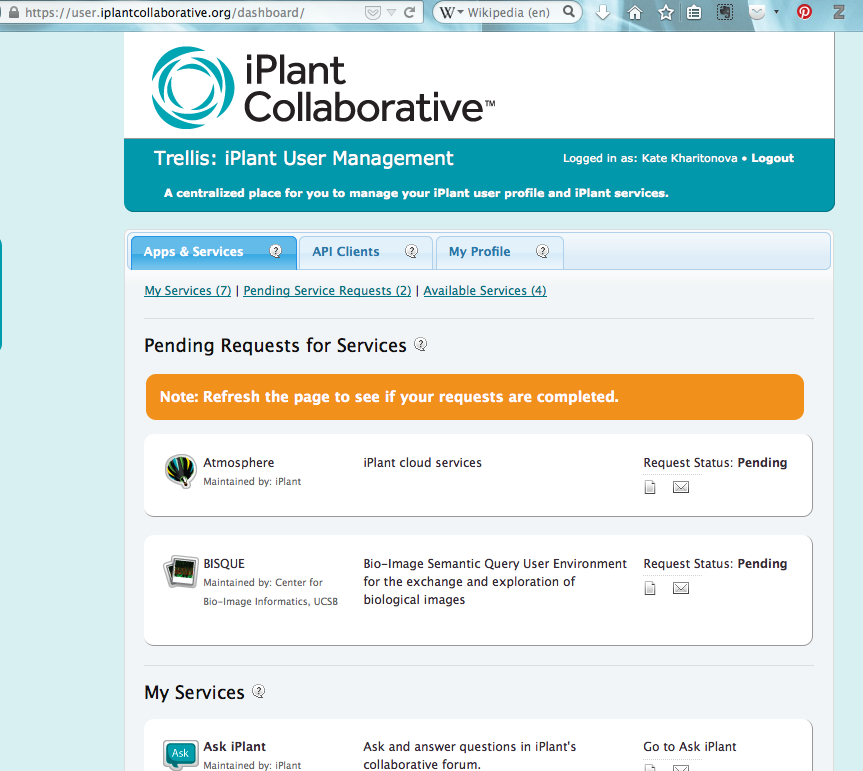
\includegraphics[width=0.6\linewidth]{./figures/pending_request.png}
  \label{fig:pending_request}
  \caption{Pending requests.}
\end{figure}

Once the request is approved, use the 
``Go to BISQUE"~\cite{Bisque-iplant} link to access the 
Bisque database hosted by iPlant.


\subsection{Analysis code}
\label{sec:analysis_code}

Select an existing program to turn into a Bisque module.
This analysis code can be written in any language, and with the help
of the Bisque API, it can be ``wrapped" and connected to the
Bisque services.

For the purposes of this tutorial, I am using a C++ program
that finds points of interest in images. 
I created an executable binary, which I can run on the command line.

\begin{verbatim}
./find_points --output-directory=$OUTDIR --has-tip-growth --min-blob-size=5 
--max-blob-size=50 --num-threads=8 $INDAT/Pos001_S001_t%02d_z%02d_ch00.tif
\end{verbatim}

The above command shows the parameters that are required
to run the code: \texttt{\$OUTDIR} is a path to an output
directory, \texttt{\$INDAT} is a path to where the input files are, 
%and \texttt{Pos001_S001_t\%02d_z\%02d_ch00}
%is the Unix printf-style pattern, which describes the format of the 
%input file names.
with the input file names described using a Unix printf-style pattern.

% -----------------------------------------------
\section{Creating a module}
\label{sec:creating-a-module}
\subsection{Overview of steps}

Following a Bisque module creation tutorial~\cite{Bisque-module-creation}, below are the steps for setting up a working module:
\begin{enumerate}
\item Create a module definition XML
\item Make the module code work with Bisque (either by modifying the module code to use the Bisque API or write a wrapper / conversion glue code)
\item Create a web server or run Engine Server
\subitem Engine Service - write configuration file on how Engine Service will run your code 
\item Register module with the Bisque system 
\end{enumerate}




% -----------------------------------------------
{\small
\bibliographystyle{abbrv}
\bibliography{references}
}
\end{document}
